
\begin{figure}
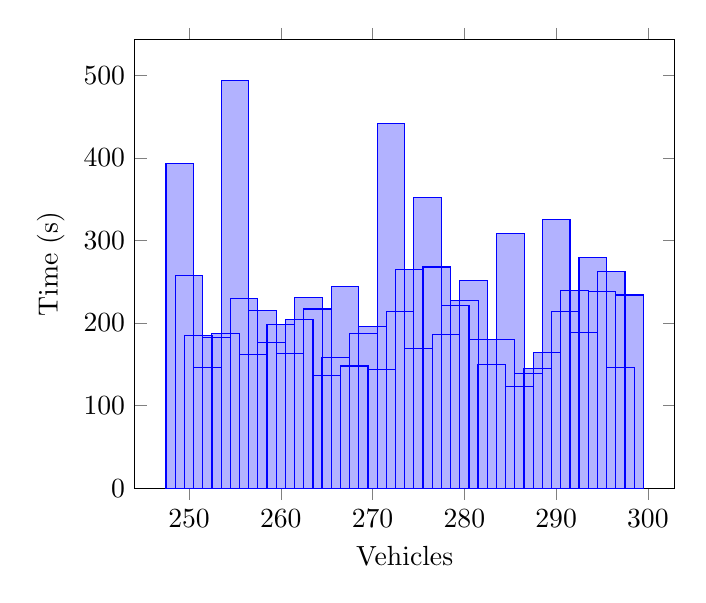
\begin{tikzpicture}
\begin{axis}[
legend style={anchor=west},
xlabel=Vehicles,
ylabel=Time (s),
ymin=0,
ybar,
]
\addplot coordinates {
(298, 234)
(296, 263)
(297, 146)
(294, 280)
(295, 238)
(292, 240)
(293, 189)
(290, 326)
(291, 214)
(270, 196)
(271, 144)
(272, 442)
(273, 214)
(274, 265)
(275, 169)
(276, 352)
(277, 268)
(278, 186)
(279, 221)
(249, 393)
(252, 146)
(258, 215)
(259, 176)
(250, 258)
(251, 185)
(256, 230)
(257, 162)
(254, 187)
(261, 163)
(289, 164)
(288, 145)
(281, 252)
(280, 227)
(282, 180)
(285, 309)
(284, 180)
(287, 139)
(286, 123)
(263, 231)
(262, 204)
(260, 198)
(267, 244)
(266, 158)
(265, 137)
(264, 217)
(269, 187)
(268, 148)
(253, 182)
(283, 150)
(255, 494)
};

\end{axis}
\end{tikzpicture}
\label{tik:time:100:91}
\caption{100 percent diving with GSC on route $91$}
\end{figure}
